\bigbreak
\subsection{Функціональні вимоги}
\bigbreak
Узагальнені варіанти використання включено до функціональних вимог та проаналізовано за принципом MoSCoW:
\begin{itemize}
 \item Життєвий цикл
 \begin{itemize}
  \item Організаційні процеси
  \begin{itemize}
   \item Навчання
   \begin{itemize}
    \item Опанування Kendo UI
   \end{itemize}
   \item Створення інфраструктури
   \item Керування проектом
  \end{itemize}
  \item Основні процеси
  \begin{itemize}
   \item Розробка
   \begin{itemize}
    \item Аналіз вимог
    \item {[}M{]} ВВ: реєстрація
    \item {[}M{]} ВВ: авторизація
    \item {[}M{]} ВВ: робота з викладачами
    \item {[}M{]} ВВ: робота з курсами
    \item {[}W{]} ВВ: робота з розкладом
    \item {[}M{]} ВВ: робота зі слухачами
    \item {[}M{]} ВВ: запис слухачів на курс
    \item {[}M{]} ВВ: робота з обліковими записами
    \item {[}C{]} ВВ: робота з коефіціентами
    \item {[}S{]} ВВ: створення звітів
    \item {[}S{]} ВВ: обробка заявок
    \item {[}M{]} ВВ: обробка облікових записів
   \end{itemize}
   \item Впровадження
  \end{itemize}
  \item Допоміжні процеси
  \begin{itemize}
   \item Документування
   \item Забезпечення якості
   \begin{itemize}
    \item Модульне тестування
    \item Тестування інтерфейсу користувача
   \end{itemize}
   \item Вирішення проблем
  \end{itemize}
 \end{itemize}
\end{itemize}
\bigbreak
\subsection{Нефункціональні вимоги}
\bigbreak
\begin{itemize}
 \item Відображати та редагувати дані, що вводяться в систему, у таблицях
 \item Відображати на екрані одну або дві різні таблиці одночасно
 \item Вкладені таблиці для сутностей, пов'язаних зв'язком M--M
 \item Гарячі клавіші для додання нового запису, видалення запису, збереження запису
 \item Підтримка стабільних версій браузерів Firefox та Chrome, Internet Explorer 8--11
 \item Час реакції $\leqslant$ 5 секунд
 \item Імовірність збою --- 0.01
 \item Підтримка резервного копіювання даних та відновлення з резервних копій
\end{itemize}
\bigbreak
\subsection{Планування розробки}
\bigbreak
Представлення: клієнт. Бізнес-логіка: сервер. Дані: БД.

Технології розробки: мова PHP5.4, СКБД MySQL 5, Web-технології, формат даних JSON.

Інструменти розробки: редактор Vim, система контролю версій Git, бібліотека тестування запитів Dogpatch.

Діаграми: рис. 3--5.

\begin{landscape}
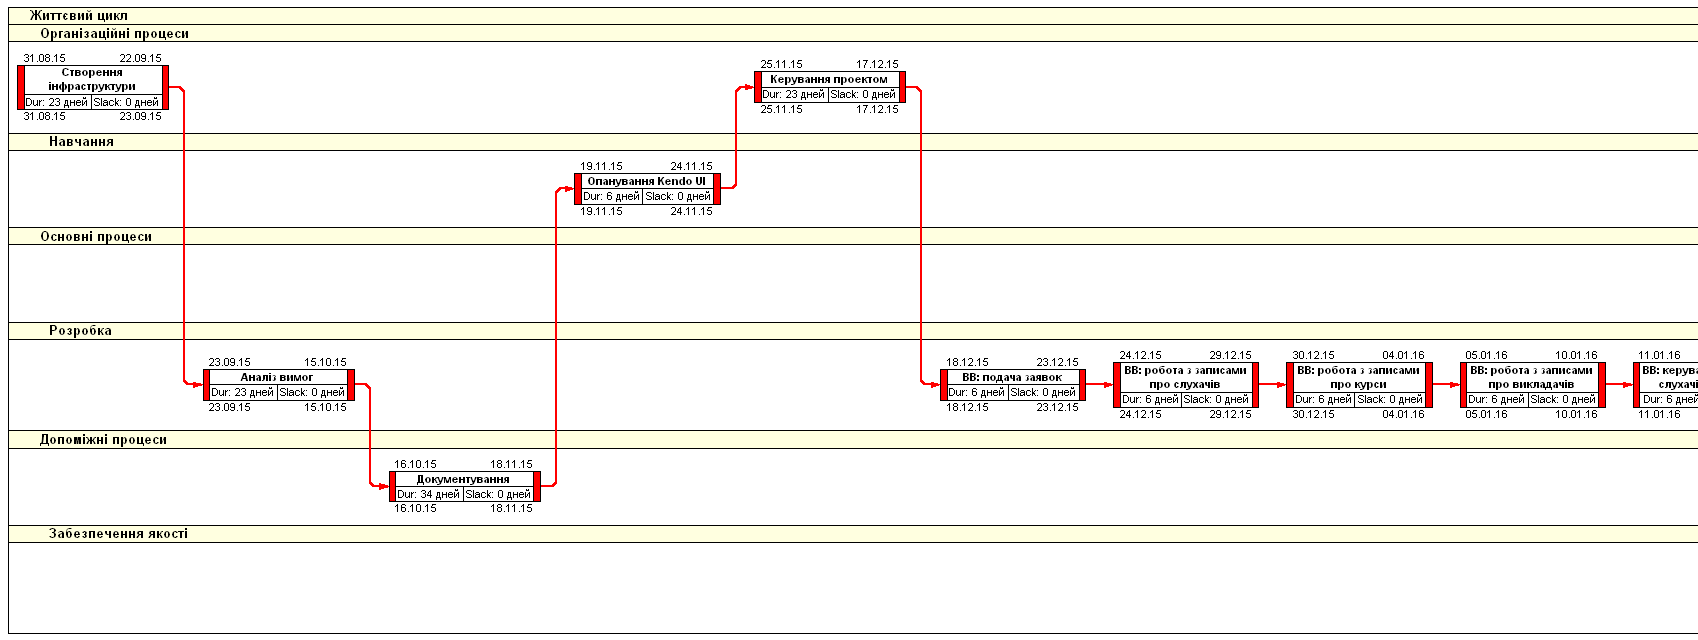
\includegraphics[width=24cm]{smp_cgw2_2.png}\\
\imglabel{Діаграма WBS}
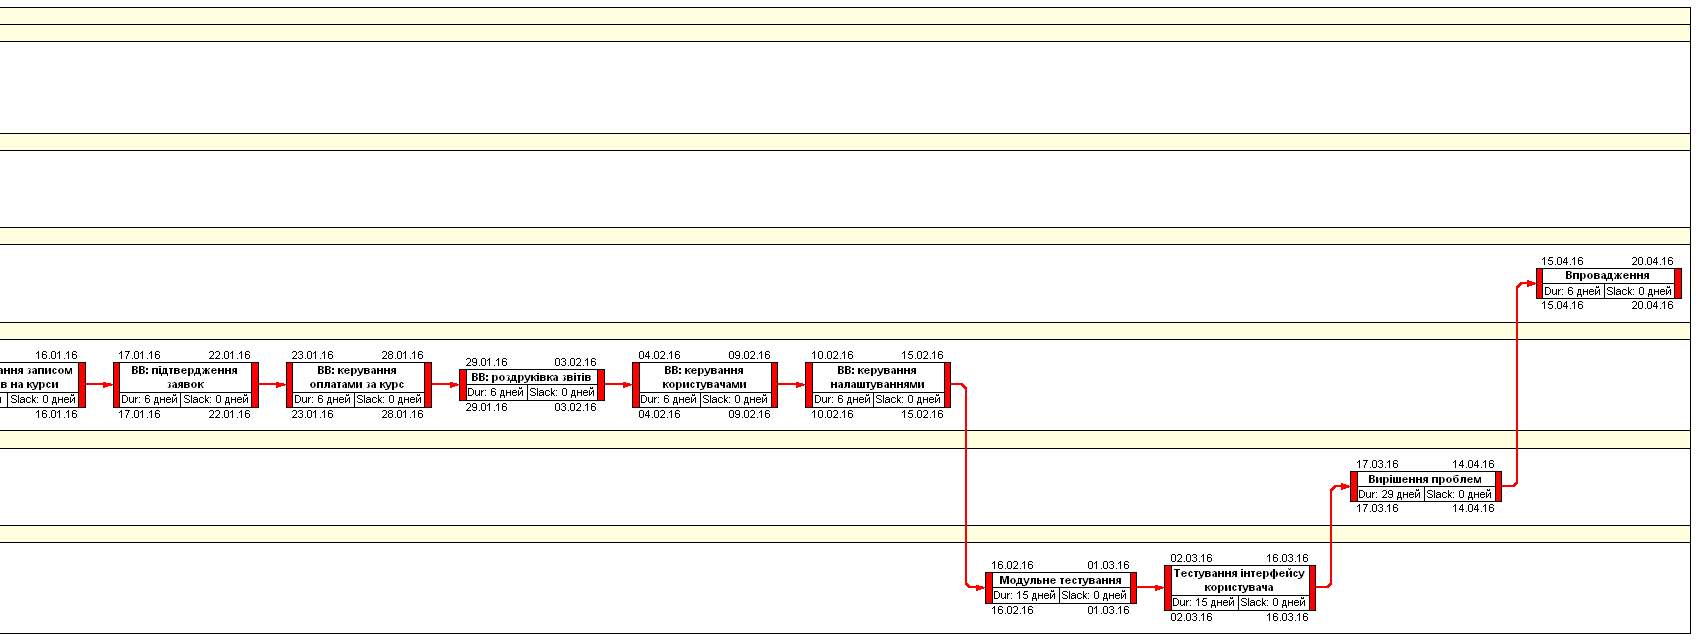
\includegraphics[width=24cm]{smp_cgw2_3.png}\\
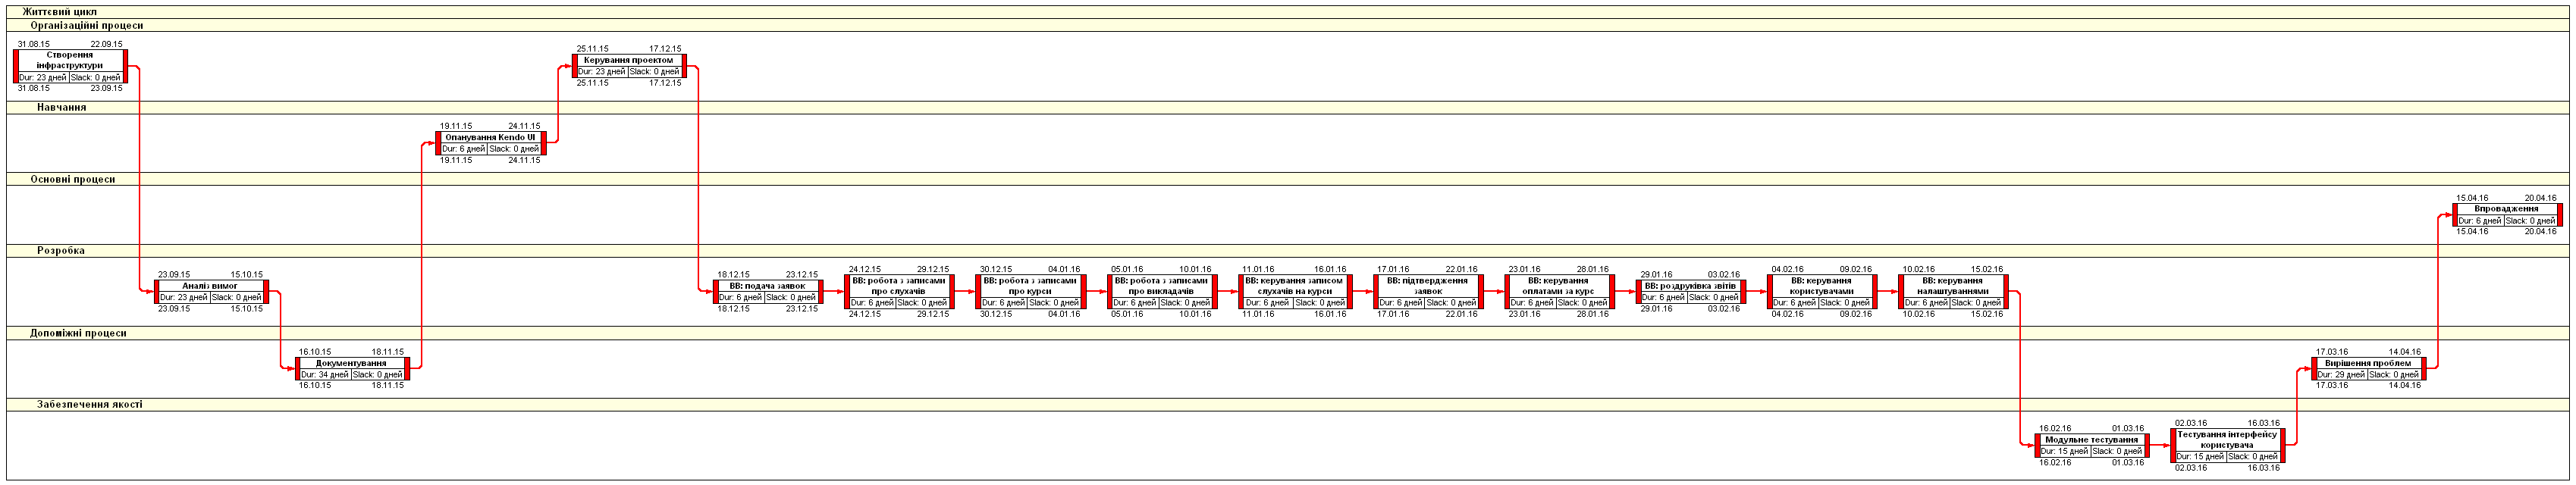
\includegraphics[width=24cm]{smp_cgw2_4.png}
\imglabel{Діаграма WBS (продовження)}
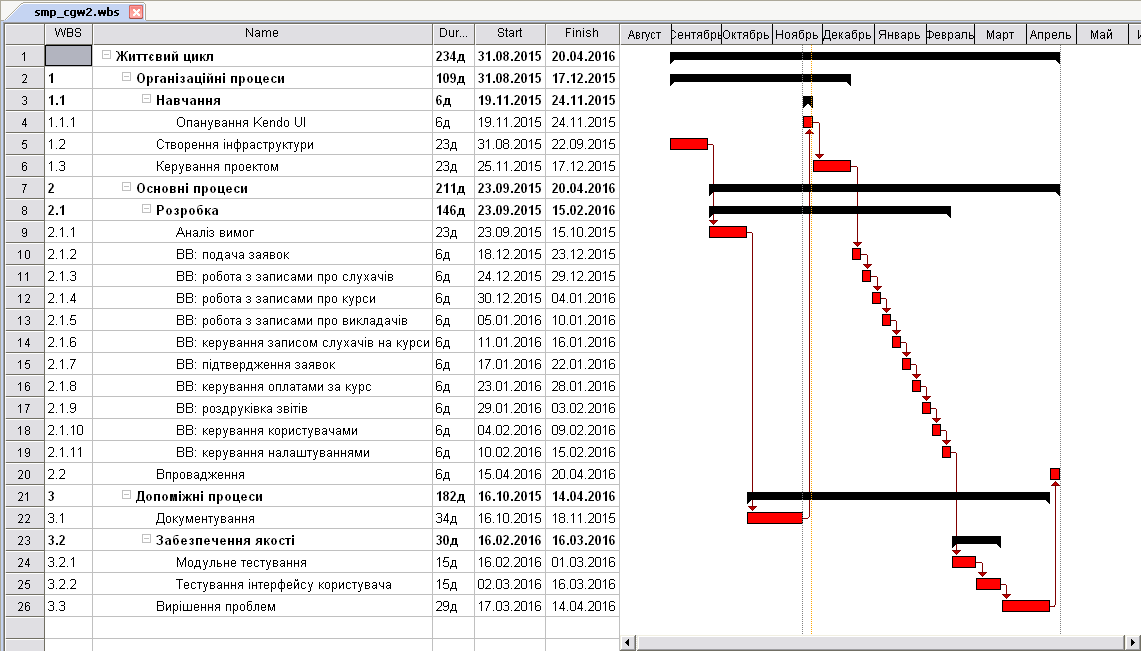
\includegraphics[width=24cm]{smp_cgw2_1.png}
\imglabel{Діаграма Ганта}
\end{landscape}
